\section{Aufgabe 2}
\subsection{Abschätzung des Arbeitswiderstandes}

Um den Arbeitswiderstand zu bestimmen, benutzen wir das Vier-Quadranten-Kennlinienfeld (Abbildung 7) und gehen vom äußersten Punkt des dritten Quadranten für \(I_B\)= 140,8\(\mu A\) senkrecht nach oben. Im Zweiten Quadranten treffen wir so den Wert für \(I_C\)=13,9 mA, welches unser Startpunkt der Arbeitsgeraden (bzw. Kollektor-Widerstandsgerade) sein wird. Damit ergeben sich die Koordinaten (\(U_{CE}\) = 0V, \(I_{C}\) = 13,9mA) für den Punkt \(P_1\) des Kurzschlussfalls. Der Punkt \(P_2\) liegt bei den Koordinaten (\(I_{C}\) = 0mA, \(U_{CE}\) = 12V), weil 12[V] die maximale Versorgungsspannung betrug.\\
Der Arbeitspunkt \(P_{A}\) liegt laut Definition bei \(\left(\frac{U_{CE}}{2}, \frac{I_{C}}{2}\right)\), welches bei uns den Werten (6.055V,6.95mA) entspricht.\\

Den Arbeitswiderstand wird über die Formel:
\begin{equation}
\notag
R_{A}=\mid \frac{1}{m}\mid = \left(\frac{U_{EC}}{I_C}\right) = 871.23 \Omega
\end{equation}\\

Während des Versuchs haben wir für den Arbeitswiderstand einen Wert von (\(464.3\pm 2.6)\Omega\) gemessen.\\

Der Basisvorwiderstand ergibt sich aus der Formel:
\begin{equation}
\notag
R_V= \frac{U_{EC}-U_{EB}}{I_B}=\frac{6V-0.7V}{(63.5\cdot 10^{-6})A}=83.5k\Omega
\end{equation}

Hier hatten wir einen Wert von (\(100.2\pm 0.8)k\Omega\) gemessen. Auf die Unterschiede dieser Werte werden wir später in der Diskussion eingehen.

\subsection{Überprüfung der Kollektor-Widerstandsgeraden}

\begin{center}
\begin{minipage}{\linewidth}
\centering
\makebox[0cm]{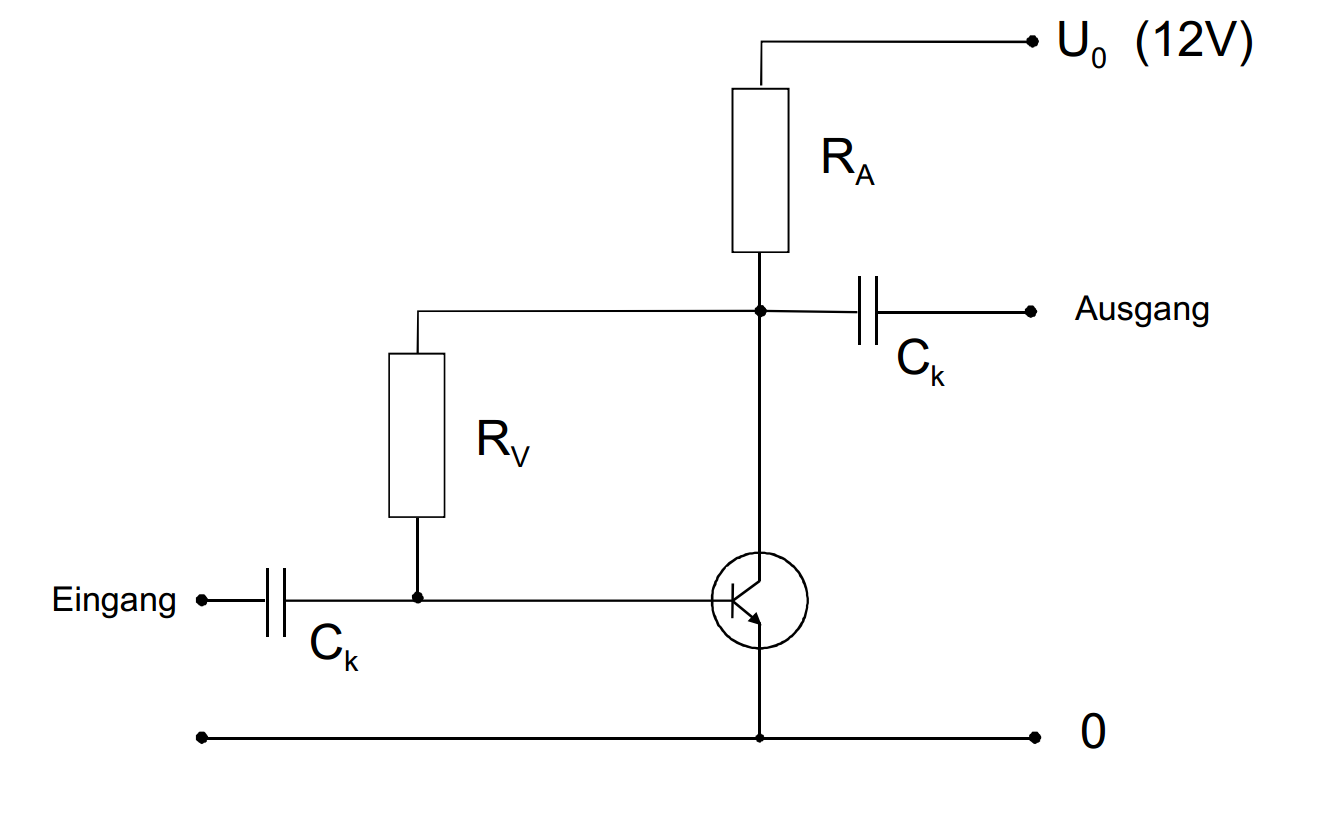
\includegraphics[width=\textwidth]{bilder/tra6}}
\captionof{figure}{Schaltplan für Aufgabe 2.2}%
\label{Schaltplan2}
\end{minipage}
\end{center}

Nun überprüfen wir die abgeschätzten Werte, indem wir einen Arbeitswiderstand und einen Basisvorwiderstand in die Schaltung einbauen (siehe Abbildung 6) und eine neue Messreihe aufnehmen. Wir steigern dabei die Werte für \(I_B\) in gleichen Abständen und notieren, wie sich die anderen Größen dazu verhalten. \(U_0\) hielten wir konstant auf (\(12.11\pm 0.09\))

Unsere Messung ergaben folgende Werte:\\

\begin{center}
\begin{tabular}{r r r r}
\(I_B [\mu A]\) & \(I_C [mA]\) & \(U_B [V]\) & \(U_{CE}[V]\) \\
\hline
\(52.116\) & \(9.0\) & \(0.116\) & \(7.93\) \\ 
\(62.519\) & \(9.3\) & \(0.191\) & \(7.75\) \\ 
\(72.518\) & \(9.7\) & \(0.255\) & \(7.59\) \\ 
\(81.305\) & \(10.0\) & \(0.315\) & \(7.45\) \\ 
\(94.132\) & \(10.5\) & \(0.362\) & \(7.22\) \\ 
\(101.505\) & \(10.9\) & \(0.429\) & \(7.01\) \\ 
\(113.423\) & \(11.8\) & \(0.526\) & \(6.61\) \\ 
\(122.311\) & \(12.6\) & \(0.586\) & \(6.24\) \\ 
\(131.906\) & \(22.7\) & \(0.755\) & \(1.52\) \\ 
\(142.410\) & \(23.4\) & \(0.757\) & \(1.17\)
\end{tabular}
\captionof{table}{Rohmesswerte für Aufgabe 2.2}
\end{center}
\newpage
Und als Vier-Quadranten-Kennlinienfeld:
\begin{center}
\begin{minipage}{\linewidth}
\centering
\makebox[0cm]{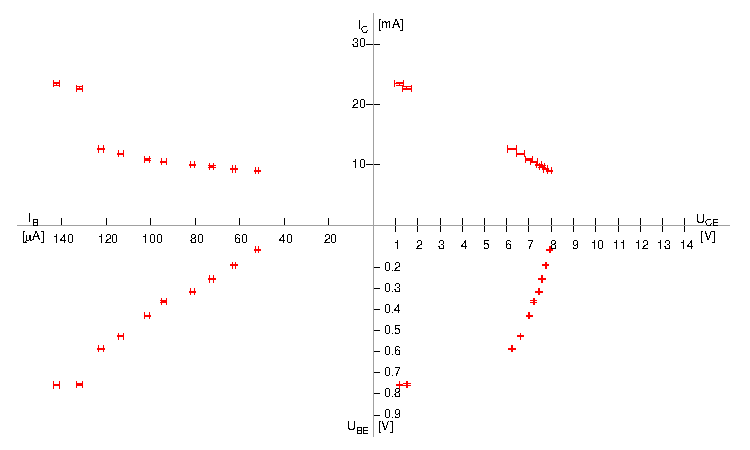
\includegraphics[width=\textwidth]{graphen/a2.pdf}}
\captionof{figure}{Kollektor-Widerstandsgerade}%
\label{dynamisches kennlinienfeld}
\end{minipage}
\end{center}

Nun tragen wir \(I_C\) gegen \(U_{CE}\) auf (Abbildung 8) um die Kollektor-Widerstandsgerade. Um die Stromverstärkung \(\beta\) zu bestimmen, plotten wir \(I_C\) gegen \(I_B\) (Abbildung 9). \(\beta\) können wir nun von der Steigung ablesen. Das Programm Mathematica liefert uns den Wert:
\begin{equation}
\notag
\beta= (124.21\pm 0.33) 
\end{equation}


\begin{center}
\begin{minipage}{\linewidth}
\centering
\makebox[0cm]{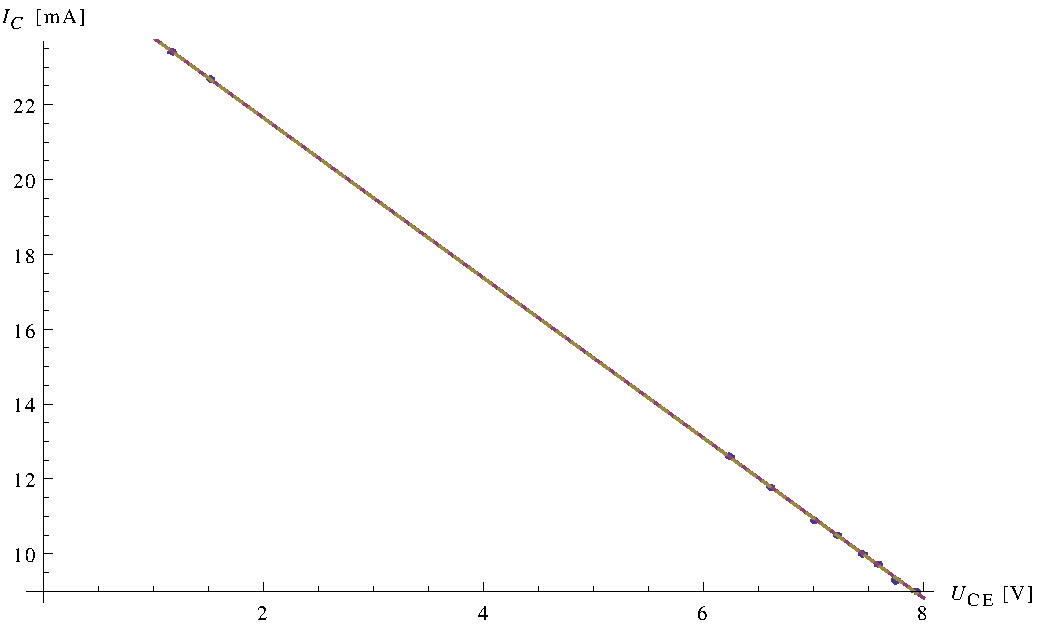
\includegraphics[width=\textwidth]{graphen/graph_2_2_1}}
\captionof{figure}{Kollektor-Widerstandsgerade}%
\label{transistor}
\end{minipage}
\end{center}

\begin{center}
\begin{minipage}{\linewidth}
\centering
\makebox[0cm]{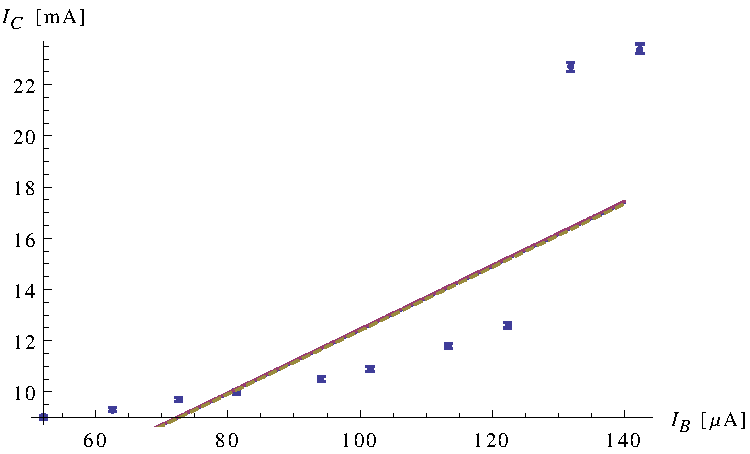
\includegraphics[width=\textwidth]{graphen/graph_2_2_2}}
\captionof{figure}{Stromverstärkung}%
\label{transistor}
\end{minipage}
\end{center}

\subsection{Verstärkung eines Sinussignals}

Nun bauen wir den Schaltplan aus Aufgabe 2.2 um und tauschen die zwei 2,2\(k\Omega\) und 22\(k\Omega\) gegen zwei 0.1\(\mu F\) Koppelkondensatoren. Die 1,5V Batterie wird gegen einen Funktionsgenerator ausgetauscht, welcher einen sinusförmigen Wechselstrom erzeugt. Über ein Oszilloskop können wir die Änderungen der Eingangs- bzw. Ausgangsspannungen beobachten. Was dabei geschieht ist folgendermaßen erklärbar:

\begin{itemize}
\item Änderung der Eingangsspannung: Die Überlagerungsspannung wurde verringert, dabei verringerte sich auch die Ausgangsspannung. Das wird dadurch verursacht, dass der Transistor bei größeren Basisspannungen auch mehr Strom auf der Kollektor-Emitter-Strecke durchlässt und somit größere Ausgangsspannungen erzeugt.
\item Änderung des Arbeitspunktes: Verringert man die Arbeitsspannung, so treten an der Basis negative Spannungen auf, diese ermöglichen jedoch keinen Strom auf der Kollektor-Emitter-Strecke und somit werden, wenn die Amplitude des Eingangssignals kleiner ist als die Arbeitsspannung, die unteren Enden der Sinusspannung abgeschnitten. Ist die Arbeitsspannung dagegen zu groß, so können irgendwann praktisch alle Elektronen die Kollektor-Emitter-Strecke passieren und eine Änderung des Eingangssignals führt zu keiner Änderung des Ausgangssignals mehr. Das bedeutet, dass die oberen Enden der Sinusspannung verzerrt werden.
\item Frequenzänderung: Änderungen der Frequenz vom Eingangssignal haben keinen Einfluss auf den Transistor, sehr wohl aber auf die Kondensatoren, deren Wechselstromwiderstand mit \(\frac{1}{\omega C}\) mit steigender Frequenz gegen 0 geht. Daher war eine steigende Verstärkung mit steigender Frequenz zu beobachten. Außerdem tritt auch eine Phasenverschiebung auf, die auch nur auf die Kondensatoren zurückzuführen ist. Diese beträgt \(\frac{\pi}{2}\). 

\end{itemize}

\subsection{Fazit}

Die geschätzte Werte für den Arbeitswiderstand und den Basisvorwiderstand weichen von den im Versuch gemessenen Werten sehr stark ab; die Werte in Abbildung 9 liegen nicht auf einer Ursprungsgeraden und zwei der Werte sind ganz verschoben. Als Fazit kann man also sagen, dass diese Messungen nicht erfolgreich verliefen. Wahrscheinliche Fehlerursachen liegen in der Qualität des Steckbrettes, welches für einige Wackelkontakte verantwortlich war. Des Weiteren lieferten uns Messgeräte vollkommen abstruse Werte und schalteten sich während der Messung ohne jeden ersichtlichen Grund einfach aus. In Abbildung \ref{dynamisches kennlinienfeld} ist auch zu sehen, dass die zwei äußersten Werte jedes Quadranten weitab von den anderen Messwerten liegen.\\

